\documentclass[conference]{IEEEtran}
\IEEEoverridecommandlockouts
% The preceding line is only needed to identify funding in the first footnote. If that is unneeded, please comment it out.
\usepackage{cite}
\usepackage{amsmath,amssymb,amsfonts}
\usepackage{algorithmic}
\usepackage{graphicx}
\usepackage{textcomp}
\usepackage{xcolor}
\usepackage{soul}
\usepackage{url}
\usepackage{tikz}
\usetikzlibrary{arrows.meta,positioning}
 
\def\BibTeX{{\rm B\kern-.05em{\sc i\kern-.025em b}\kern-.08em
    T\kern-.1667em\lower.7ex\hbox{E}\kern-.125emX}}
\begin{document}
 
\title{Simulation-Driven Benchmarking Framework for LiDAR-Based Collision Avoidance on AGVs}
 
\author{
\IEEEauthorblockN{
		Myroslav Mishchuk$ ^{1,2}$,
        Leonardo Schiavo$^{3} $,
		Milad Jafari Barani$^{4}$,
        S M Asiful Huda$^{5} $, and
        Rafał Cupek$^{1}$
        }
	\IEEEauthorblockA{$ ^{1} $Silesian University of Technology, Poland} 
    \IEEEauthorblockA{$ ^{2} $Lviv Polytechnic National University, Ukraine} 
    \IEEEauthorblockA{$ ^{3} $Universidad Politécnica de Madrid, España} 
    \IEEEauthorblockA{$ ^{4} $University of Oviedo, Spain} 
    \IEEEauthorblockA{$ ^{5} $University of Naples Federico II, Italy} 
}
\maketitle

\begin{abstract}
LiDAR-based collision avoidance for automated guided vehicles (AGVs) is commonly evaluated using custom scenarios, simulation setups, and metrics. The absence of a standardized evaluation framework makes cross-study comparison and results reproduction difficult. In this paper, we introduce a simulation-driven benchmarking framework for LiDAR-based AGV collision avoidance. The framework combines a parameterized procedural world generator with a modular three-stage simulation engine (detection, fusion, avoidance) and an explicit LiDAR and prior-map degradation model. We validate the framework on a stratified corpus of 480 worlds spanning 48 strata, executing 11,520 simulation runs over eight algorithm pipelines and three sensor configurations. The results indicate that the corpus is well-formed (mean free-space ratio 0.942, 0.925, 0.912 for subdivision levels 1, 2, 3, showing that higher subdivision levels produce more constrained environments; 99.8\% of worlds satisfy the clearance bound); the three-stage decomposition exhibits the intended direct-sensitivity pattern and the predicted fusion--avoidance interaction; and pipeline rankings are robust under seed resampling (mean Kendall tau 0.737) and largely stable across sensor/map degradation (mean 0.560), with one metric showing regime-dependent sensitivity that the benchmark localizes explicitly. The framework provides a reproducible, stage-addressable benchmark that isolates each algorithmic choice under controlled perception conditions, enabling cross-study comparison that ad-hoc evaluation practice currently precludes.
\end{abstract}

\vspace{-3pt}

\begin{IEEEkeywords}
Automated Guided Vehicles (AGVs), collision avoidance, benchmarking framework, LiDAR-based navigation 
\end{IEEEkeywords}
 
\section{Introduction}
\label{sec:introduction}
 
Automated Guided Vehicles (AGVs) are widely used in warehouse and manufacturing environments for material transportation, where they increasingly share floor space with human workers~\cite{fragapane2021planning}. Reliable collision avoidance is the foundational safety mechanism for human--AGV coexistence: failures translate directly into worker-injury risk, and driverless industrial trucks are accordingly governed by dedicated safety standards~\cite{iso3691-4}.
AGVs operating in dynamic environments must detect and avoid obstacles such as other vehicles, personnel, and misplaced goods in real time, typically using LiDAR as the primary perception sensor.

A substantial number of papers have been published on collision avoidance for mobile robots with a variety of algorithms proposed at each pipeline stage: obstacle detection via point cloud clustering~\cite{rusu2011pcl}, temporal fusion via tracking filters~\cite{welch1995kalman}, and local avoidance via reactive planners~\cite{borenstein1991vfh, fox1997dwa}. More recently, deep reinforcement learning (DRL) methods have been applied to end-to-end collision avoidance~\cite{qin2023endtoend}.
However, a persistent problem in this field is the lack of a standardized evaluation methodology. Each study constructs its own simulation environment, defines its own scenarios, and selects its own metrics, making cross-study comparison unreliable. Adjacent domains have addressed this through shared benchmarks: KITTI~\cite{geiger2012kitti} and nuScenes~\cite{caesar2020nuscenes} for autonomous driving perception, RWARE~\cite{papoudakis2021benchmarking} for multi-robot warehouse coordination, and BARN~\cite{perille2020barn} for metric ground navigation in cluttered spaces. But, to our knowledge, no equivalent benchmark exists for LiDAR-based AGV collision avoidance as a decomposable perception-to-action task with explicit sensor- and map-quality control.
Without a shared evaluation framework, it is impossible to determine whether a reported improvement stems from the proposed algorithm or from favorable scenario selection. Researchers cannot reproduce each other's results, and practitioners cannot make informed decisions about which collision avoidance approach to deploy.

In this paper, we propose a simulation-driven benchmarking framework that fills this gap for LiDAR-based AGV collision avoidance. The framework provides (1) a parameterized \textbf{world generator \texttt{(WG)}} that procedurally produces diverse AGV environments, with control over environment structure, obstacle configurations, and AGV mission parameters; and (2) a modular \textbf{simulation engine \texttt{(SE)}} with a formally defined perception model and pipeline decomposition, enabling controlled substitution and ablation of methods at each stage.
To validate the framework, we address the following research questions (RQs):
 
\begin{itemize}
    \item \textbf{RQ1:} Does the world generation procedure produce environments that are structurally representative of real AGV operating conditions?
    \item \textbf{RQ2:} Does the pipeline decomposition enable isolated comparison of algorithmic choices at each stage?
    \item \textbf{RQ3:} Are benchmarking results reproducible and stable across seeds, sensor configurations, and map conditions?
\end{itemize}
 
The framework is released as open source\footnote{Source code, world corpus, simulation reports, and analysis scripts: \mbox{\url{https://github.com/Myroslav437/AGV-CABench}}.} to support reproduction, extension, and cross-study comparison.
 
\section{Related Works}
\label{sec:related-works}
Industrial mobile robot navigation systems are typically structured as modular pipelines of independent stages. End-to-end approaches that map sensor inputs directly to control actions are an active research direction. However, learned policies pose challenges related to opacity, non-determinism, and verifiability that complicate compliance with safety-critical standards for driverless industrial trucks~\cite{iso3691-4, perezcerrolaza2024aisafety}. Modular pipelines, therefore, remain a popular and practical choice in industrial AGV deployments: frameworks such as ROS2 Nav2~\cite{macenski2023ros2nav} expose each stage as a configurable plugin with well-defined interfaces (for example, costmap layers for perception, pluggable global and local planners for path planning, and controller plugins for motion execution). This lets individual components be tuned, swapped, or validated in isolation, and lets learned methods be introduced at a single stage without replacing the surrounding pipeline.
 
Within this architecture, LiDAR-based obstacle detection typically relies on point cloud clustering. Euclidean clustering~\cite{rusu2011pcl} groups points using a fixed distance threshold and is widely used in AGV applications due to its simplicity and low computational cost. DBSCAN~\cite{ester1996dbscan} and its variants (HDBSCAN, OPTICS) offer greater robustness to noise and varying obstacle densities through neighborhood-based clustering criteria. At the temporal fusion level, Kalman filtering (KF)~\cite{welch1995kalman} remains the standard method for tracking detected obstacles across time steps, maintaining position and velocity estimates under noisy observations.
 
At the reactive planning level, two families dominate. The Vector Field Histogram (VFH)~\cite{borenstein1991vfh} and its successors (VFH+, VFH*) construct polar histograms of obstacle density around the robot and select the best traversable direction. The Dynamic Window Approach (DWA)~\cite{fox1997dwa} samples velocity pairs within the robot's kinematic constraints, simulates short-horizon trajectories, and selects the one maximizing a weighted objective of heading, clearance, and speed. Both are extensively deployed in AGV navigation~\cite{katona2024obstacle, pavliuk2026agv} and available in standard robotics middleware. More recently, DRL methods have been applied to collision avoidance~\cite{qin2023endtoend}.
 
A persistent issue across the collision avoidance literature is the absence of standardized evaluation methodology. Each study evaluates its proposed algorithm in a custom simulation, typically a small set of hand-designed scenarios in Gazebo, Gym, or a custom engine, with idiosyncratic metrics and environmental configurations. This ad-hoc practice is widely reported: Perille et al.~\cite{perille2020barn} observe that navigation systems are routinely compared in one or two manually chosen environments of unquantified difficulty; recent DRL navigation surveys note that evaluations are confined to simplified dynamic scenarios with inconsistent metrics~\cite{sensors2025drl_survey}; and researchers at the U.S.\ National Institute of Standards and Technology (NIST) have explicitly called for standard benchmarking procedures in their assessment of AGV navigation performance~\cite{bostelman2015navigation}.
Consequently, when studies report different performance across algorithms, it is difficult to determine whether the differences reflect algorithmic capability or favorable scenario selection. Small scenario counts further limit statistical power, leaving results incomparable across studies.
 
Adjacent domains have addressed this gap through shared benchmarks. In autonomous driving, KITTI~\cite{geiger2012kitti} and nuScenes~\cite{caesar2020nuscenes} provide standardized datasets, metrics, and leaderboards for perception tasks. In multi-robot coordination, RWARE~\cite{papoudakis2021benchmarking} provides a parameterized warehouse environment for evaluating multi-agent DRL. The closest prior work on ground navigation is BARN~\cite{perille2020barn}, which procedurally generates cluttered 2D environments via cellular automaton inspired by search-and-rescue scenarios and scores each as a monolithic sense-plan-act unit with a single learned difficulty value. However, none of these targets LiDAR-based AGV collision avoidance specifically: BARN abstracts away sensing; the autonomous-driving benchmarks address perception in isolation rather than closed-loop avoidance; and RWARE abstracts away both sensing and low-level control.
 
Our framework instead targets warehouse-style AGV operating conditions and decomposes the pipeline into detection, fusion, and avoidance stages, with explicit LiDAR and prior-map quality parameters. This enables per-stage diagnosis of failures under controlled sensor and map degradation. Crucially, the framework is a formal specification rather than a fixed dataset: world state, perception, and the simulation step are abstract interfaces independent of any particular physics backend. This allows a richer parameter space and on-demand corpus generation at an arbitrary scale.
 
 
\section{Framework Overview}
\label{sec:framework-overview}
Addressing the gap identified in Section~\ref{sec:related-works} requires an evaluation framework that specifically targets LiDAR-based collision avoidance and replaces custom, ad-hoc simulations with standardized scenarios and comparable metrics. We propose such a framework, decoupling world generation, perception-limited simulation, and algorithmic evaluation into independent, composable stages. This separation enables systematic comparison of different algorithm configurations across a large and diverse set of procedurally generated environments.
The framework consists of two principal components:
\begin{enumerate}
    \item \textbf{\texttt{WG}} --- responsible for producing a large corpus of initial world states with varying environment structures, obstacle configurations, and predefined AGV paths, governed by a rich set of generation parameters.
    \item \textbf{\texttt{SE}} --- responsible for executing step-wise simulation of the perception-limited AGV navigating through a given world under a specified algorithmic pipeline and sensor configuration, and collecting performance metrics.
\end{enumerate}
\noindent Both components are fully parameterized, enabling controlled experimentation over generation conditions, sensor characteristics, and algorithmic configurations simultaneously.
 
\subsection{Formal Definitions}
\label{sec:formal-definitions}
 
\subsubsection{Waypoint Path}
\label{sec:waypoint-path}
describes how an entity is intended to move through the environment: an ordered sequence of positions to visit, with a target speed for each segment. We define the space of waypoint paths $\mathbb{W}$ as follows. A waypoint path $\mathcal{W} \in \mathbb{W}$ is a tuple:
\begin{equation}
\label{eq:waypoint-path}
    \mathcal{W} = \big( \mathbf{w}_0,\; \mathbf{w}_1,\; \ldots,\; \mathbf{w}_n \;;\; v_1,\; v_2,\; \ldots,\; v_n \big),
\end{equation}
where:
\begin{itemize}
    \item $\mathbf{w}_j \in \mathbb{R}^2$ for $j = 0, 1, \ldots, n$ are the waypoint positions, defining $n$ straight-line segments.
    \item $v_j \in \mathbb{R}^+_0$ for $j = 1, 2, \ldots, n$ is the target speed for segment $j$, i.e., the segment from $\mathbf{w}_{j-1}$ to $\mathbf{w}_j$.
\end{itemize}
We write $|\mathcal{W}| = n$ for the number of segments. The entity following the path traverses the waypoints in order, moving along the segment from $\mathbf{w}_{j-1}$ to $\mathbf{w}_j$ at target speed $v_j$. The heading along segment $j$ is determined by the segment direction: $\theta_j = \mathrm{atan2}(\mathbf{w}_j - \mathbf{w}_{j-1})$. The trivial case $|\mathcal{W}| = 0$ represents a stationary entity. Higher-level path shapes can be approximated by denser waypoint sequences.
 
\subsubsection{Obstacle Model}
\label{sec:obstacle-model}
Each obstacle $o_i$ represents an entity in the environment that the AGV must detect and react to \emph{at runtime}. An obstacle is defined as:
\begin{equation}
\label{eq:obstacle}
    o_i = \langle S_i,\; \xi_i \rangle,
\end{equation}
where:
\begin{itemize}
    \item $S_i \subset \mathbb{R}^2$ is the spatial extent of the obstacle: a compact, closed region representing the physical space it occupies. Formally, $S_i$ is defined relative to the obstacle's centroid by its boundary:
    \begin{equation}
    \label{eq:spatial-descriptor}
        \partial S_i = (\mathbf{b}_1,\; \mathbf{b}_2,\; \ldots,\; \mathbf{b}_{n_i}),
    \end{equation}
    where $\mathbf{b}_k \in \mathbb{R}^2$ are vertices of a closed polygon expressed in the obstacle's local coordinate frame.
    \item $\xi_i \in \mathbb{W}$ is the trajectory of the obstacle's centroid.
\end{itemize}
The definition $o_i$ is fixed at the world generation stage. During simulation, the obstacle's state evolves as it progresses along its trajectory. 
The full obstacle set with time-varying states is:
\begin{equation}
\label{eq:obstacle-set}
    O_t = \{(o_i,\; \tau_i(t))\}_{i=1}^{k},
\end{equation}
where $\tau_i(t) \in [0, |\xi_i|]$ is the progress of obstacle $i$ along $\xi_i$ at time $t$, which determines its current position and heading.  
For static obstacles ($|\xi_i| = 0$), $\tau_i(t) = 0\;\;\forall\, t$. 
 
 
\subsubsection{Environment Structure}
\label{sec:environment-structure}
The environment structure $E$ represents the static, a priori known physical layout of the operating space, such as walls, columns, shelving units, and other permanent features that define the facility in which the AGV operates. Formally:
\begin{equation}
\label{eq:environment}
    E = \{e_1,\; e_2,\; \ldots,\; e_l\},
\end{equation}
where each $e_j$ is a closed polygonal chain in $\mathbb{R}^2$, representing a contiguous region of occupied space. Elements of $E$ are permanent, known before the AGV begins its mission, and available to the navigation system as part of the prior map.
 
\subsubsection{Prior map}
\label{sec:prior-map}
The prior map $M_0$ encodes the AGV's a priori knowledge of the environment, derived from the environment structure $E$ via a degradation function $\mathcal{P}$:
\begin{equation}
\label{eq:perceived-prior-map}
    M_0 = \mathcal{P}(E,\; \eta_{\text{cpl}},\; \sigma_{\text{map}}),
\end{equation}
where $\eta_{\text{cpl}} \in [0,1]$ controls map completeness (the fraction of boundary elements retained) and $\sigma_{\text{map}} \geq 0$ controls positional noise applied to retained elements. With $\eta_{\text{cpl}} = 1$ and $\sigma_{\text{map}} = 0$, $M_0$ is a copy of $E$. The degradation parameters are part of the simulation configuration. 
 
The prior map degradation is distinct from LiDAR distortion ($\Lambda_{\mathcal{D}}$). LiDAR noise is local and transient: it affects the current scan and can be filtered over time. Map errors are persistent and structural: a missing wall causes the AGV to plan routes through blocked spaces, and a shifted wall triggers false obstacle detections. These failures affect every decision throughout the mission and cannot be compensated by LiDAR alone, particularly in occluded regions outside the sensor's field of view (FOV).
The prior map is computed once at the start of each simulation run and does not change over time.
 
\subsubsection{LiDAR Scan}
\label{sec:lidar-Scan}
 
The \emph{ideal scan} at time $t$ is a discretized, range-limited slice of the physical environment as seen from the AGV's current pose:
\begin{equation}
\label{eq:ideal-scan}
    L_t^{\circ} = \mathcal{S}(E,\; O_t,\; P_t,\; \theta_t,\; \Lambda_{\mathcal{S}}) = \{(r_j,\, \alpha_j)\}_{j=1}^{N_{\text{rays}}},
\end{equation}
where:
\begin{itemize}
    \item $P_t \in \mathbb{R}^2$ is the position of the AGV (centroid) at time $t$.
    \item $\theta_t \in [0, 2\pi)$ is the heading of the AGV at time $t$.
    \item $\Lambda_{\mathcal{S}}$ is LiDAR sensor parameters (see Section~\ref{sec:lidar-params}). 
\end{itemize}
For each ray at angle $\alpha_j$ relative to the heading, $r_j$ is the true distance to the nearest surface, whether belonging to $E$ or to an obstacle in $O_t$. The scan function $\mathcal{S}$ returns perfect, noise-free measurements.
 
Real LiDAR hardware introduces noise, missed detections, and spurious readings. The distortion function $\mathcal{D}$ transforms the ideal scan into a "realistic" one:
\begin{equation}
\label{eq:distorted-scan}
     \hat{L}_t = \mathcal{D}(L_t^{\circ},\; \Lambda_{\mathcal{D}})
    = \{(\hat{r}_j,\, \alpha_j)\}_{j=1}^{N_{\text{rays}}},
\end{equation}
where $\Lambda_{\mathcal{D}}$ are the LiDAR distortion parameters (see Section~\ref{sec:lidar-params}). The LiDAR observes both obstacles and environment structure indiscriminately.
 
\subsubsection{World State}
\label{sec:world-state}
A world state at time $t$ is defined as the tuple:
\begin{equation}
\label{eq:world-state}
    W_t = \langle E,\; O_t,\; \pi,\;  P_t,\; S_{\text{agv}},\; \theta_t,\; \mathbf{v}_t \rangle,
\end{equation}
where:
\begin{itemize}
    \item $\pi \in \mathbb{W}$ is the time-invariant AGV's reference path that the AGV is expected to follow in the absence of obstacles~\eqref{eq:waypoint-path}. The first waypoint $\mathbf{w}_0$ of $\pi$ is the start position; the last waypoint $\mathbf{w}_n$ is the goal.
    \item $S_{\text{agv}} \subset \mathbb{R}^2$ is the time-invariant spatial extent of the AGV (same as \eqref{eq:spatial-descriptor}).
    \item $\mathbf{v}_t \in \mathbb{R}^2$ is the velocity vector of the AGV at time $t$.
\end{itemize}
The world state is an "objective" representation of the physical environment and the AGV's mission: it describes what exists and what the AGV is tasked to do, independent of what the AGV perceives or believes at runtime.
  
  
\subsubsection{Perception Model}
\label{sec:perception-model}
The AGV does not have direct access to the "objective" world state $W_t$. Instead, it operates on a perceived world $\tilde{W}_t$:
\begin{equation}
\label{eq:perception-function}
    \tilde{W}_t = \Psi(W_t)
    = \langle M_0,\; \pi,\; S_{\text{agv}},\; \hat{L}_t,\; P_t,\; \theta_t,\; \mathbf{v}_t \rangle,
\end{equation}
where $\Psi$ is a perception function that transforms the objective world through the sensors and prior knowledge. We assume the AGV has perfect knowledge of its own pose: $P_t$, $\theta_t$, $\mathbf{v}_t$ pass through $\Psi$ unchanged. Relaxing this assumption is left to future work (Section~\ref{sec:discussion}).
 
% ============================================================
\subsection{World Generator (\texttt{WG})}
\label{sec:world-generator}
 
 
The \texttt{WG} constructs initial world states $W_0$.  A single world is generated as:
\begin{equation}
\label{eq:generation}
    \texttt{WG}(\Omega,\; s_{\text{wg}}) \to W_0,
\end{equation}
where \texttt{WG} is presented as stochastic generation function parameterized by a parameter set $\Omega$ and seeded by $s_{\text{wg}} \in \mathbb{N}$, which initializes the pseudo-random number generator:
\begin{equation}
\label{eq:omega}
    \Omega = \langle \Omega_{\text{env}},\; 
    \Omega_{\text{agv}},\;
    \Omega_{\text{path}}, \; 
    \Omega_{\text{obs}} \rangle.
\end{equation}
 
The generation proceeds in five stages: (1)~the environment structure $E$ is generated via \emph{Binary Space Partitioning} (BSP) from $\Omega_{\text{env}}$; (2)~the AGV spatial extent $S_{\text{agv}}$ is constructed from $\Omega_{\text{agv}}$; (3)~the AGV reference path $\pi$ is generated via \emph{Probabilistic Roadmap} (PRM) within the free space of $E$ according to $\Omega_{\text{path}}$; (4)~static and dynamic obstacles are placed in the free space of $E$ according to $\Omega_{\text{obs}}$, respecting clearance constraints relative to boundary geometry and the reference path; (5)~trajectories for dynamic obstacles are generated via PRM within the free space of $E$.
The corpus of $N$ initial worlds is produced using \texttt{WG}:
\begin{equation}
\label{eq:corpus}
    \mathcal{C} = \{W_0^{(i)}\}_{i=1}^{N}, \quad N = 480.
\end{equation}
To ensure coverage over the parameter space, the corpus is stratified: $\Omega$ is systematically varied across predefined ranges (see Section~\ref{sec:experimental-design}), so that each region of the parameter space is represented by a sufficient number of worlds.
 
 
\subsubsection{Environment parameters $\Omega_{\text{env}}$}
These parameters control the generation of the environment structure $E$. The generation of boundary geometry depends on the chosen spatial partitioning algorithm; in this work, we employ BSP, a well-established recursive subdivision method widely used in procedural environment generation~\cite{shaker2016pcg}. The BSP algorithm recursively divides the environment into axis-aligned rectangular partitions; boundary elements (walls) are placed along partition edges, and rooms or passages are carved within leaf partitions. By varying the BSP parameters, a single algorithm produces structurally diverse layouts, from open spaces to dense room-based facilities.
The environment parameters are:
\begin{itemize}
    \item $X, Y \in \mathbb{R}^+$ --- spatial dimensions of the environment.
    \item $d_{\text{bsp}} \in \mathbb{N}^+$ --- the number of recursive subdivision levels. Low values (1--2) yield open layouts with few large partitions; medium values (3--4) produce corridor- or aisle-like structures; high values (5+) generate dense, room-based environments.
    \item $s_{\min}^{w},\; s_{\min}^{h} \in \mathbb{R}^+$ --- the smallest allowable width and height for a leaf partition. These prevent degenerate (too narrow or too small) regions and indirectly control room size.
    \item $\rho_{\text{split}} \in [\rho_{\min},\; \rho_{\max}] \subset (0, 1)$ --- split ratio range. Narrow ranges (e.g., $[0.45, 0.55]$) produce regular, aisle-like partitions; wide ranges (e.g., $[0.2, 0.8]$) produce heterogeneous room sizes.
    \item $p_{\text{room}} \in [p_{\min},\; p_{\max}] \subset [0, 1)$ --- room padding range. Low padding yields rooms that nearly fill their partitions (dense layout); high padding yields smaller rooms with more open space.
    \item $c_{\min} \in \mathbb{R}^+$ --- minimum corridor width between adjacent boundary elements (room walls and partition walls).
    \item $w_{\text{pass}} \in \mathbb{R}^+$ --- the width of corridors connecting sibling partitions. Controls navigability and the effective aisle width.
    \item $t_{\text{wall}} \in \mathbb{R}^+$ --- the thickness of boundary elements placed along partition edges and room perimeters.
\end{itemize}
The BSP algorithm outputs a set of closed polygonal chains (the walls and room boundaries), which constitutes the environment structure $E$. Different parameter configurations are used to stratify the world corpus across layout types (see Section~\ref{sec:experimental-design}).
 
\subsubsection{AGV parameters $\Omega_{\text{agv}}$}
These parameters define the physical properties of the AGV: the body length $L_{\text{agv}} \in \mathbb{R}^+$ and body width $W_{\text{agv}} \in \mathbb{R}^+$.
 
\subsubsection{Path parameters $\Omega_{\text{path}}$}
These parameters control the generation of the reference path $\pi \in \mathbb{W}$. As with environment generation, path generation depends on the chosen algorithm; in this work, we employ the PRM method, a well-established sampling-based path planning algorithm widely used in robotics~\cite{lavalle2006planning}.
The path generation proceeds as follows: (1)~inflate the boundary elements of $E$ by a clearance margin $d_{\text{clear}}$; (2)~sample $n_{\text{samples}}$ random points in the inflated free space; (3)~connect each sample to its $k_{\text{nn}}$ nearest neighbors via collision-free straight-line edges; (4)~sample start and goal positions in the free space; (5)~insert start and goal into the roadmap and find the shortest path via Dijkstra's algorithm; (6)~assign target speeds to each segment from $\mathcal{D}_{v^\star}$.
The path parameters are:
\begin{itemize}
    \item $n_{\text{samples}} \in \mathbb{N}^+$ --- number of random points sampled in the free space (controls roadmap density and path diversity).
    \item $k_{\text{nn}} \in \mathbb{N}^+$ --- number of nearest neighbors to attempt connections with (controls roadmap connectivity).
    \item $l_{\max} \in \mathbb{R}^+$ --- maximum edge length; connections longer than $l_{\max}$ are rejected.
    \item $d_{\text{clear}} \in \mathbb{R}^+$ --- wall clearance distance (obstacle inflation radius); the generated path is guaranteed to maintain at least this distance from any boundary element in $E$.
    \item $l_{\pi}^{\min} \in \mathbb{R}^+$ --- minimum path length.
    \item $\mathcal{D}_{v^\star}$ --- distribution over target segment speeds (e.g., $\mathrm{Uniform}(v_{\min}^{\star}, v_{\max}^{\star})$, or constant speed across all segments).
\end{itemize}
 
\subsubsection{Obstacle parameters $\Omega_{\text{obs}}$}
These parameters control the generation of the obstacle set $O_{t=0}$. In the current implementation, obstacle shapes are restricted to circles and squares, both parameterized by a single scalar: the inscribed circle radius $r_i$.
Trajectories for dynamic obstacles are generated using the same PRM-based approach as the AGV reference path, with their own parameter set. The complete parameter set for obstacles is:
\begin{itemize}
    \item $n_{\text{static}}\in \mathbb{N}$ --- number of static obstacles.
    \item $n_{\text{dynamic}}\in \mathbb{N}$ --- number of dynamic obstacles.
    \item $\mathcal{D}_{r}$ --- distribution over inscribed circle radius (e.g., $\mathrm{Uniform}(r_{\min}, r_{\max})$). For circles, $r_i$ is the radius directly; for squares, $r_i$ is the half-side length (the radius of the inscribed circle).
    \item $d_{\min}$ --- minimum clearance between any two obstacle boundaries and between obstacles and environment boundary geometry.
    \item $n_{\text{samples}}^{\text{obs}}$, $k_{\text{nn}}^{\text{obs}}$, $l_{\max}^{\text{obs}}$, $d_{\text{clear}}^{\text{obs}}$ --- PRM roadmap parameters for obstacle trajectory generation (analogous to the AGV path parameters; may differ to produce shorter or less constrained paths).
    \item $\mathcal{D}_{v}^{\text{obs}}$ --- distribution over segment target speeds for dynamic obstacles (e.g., $\mathrm{Uniform}(v_{\min}, v_{\max})$).
\end{itemize} 
 
For static obstacles, the trajectory is simply a single waypoint at the obstacle's initial position: $\xi_i = (\mathbf{w}_0)$ with $|\xi_i| = 0$.
 
% ============================================================
\subsection{Simulation Engine (\texttt{SE})}
\label{sec:simulation-engine}
Each simulation run is fully specified by:
\begin{equation}
\label{eq:invocation}
    \texttt{SE}(W_0,\; \mathcal{A},\; \Sigma,\; s_{\text{se}}) \to \mathcal{M},
\end{equation}
where $W_0 \in \mathcal{C}$ is an initial world from the generated corpus, $\mathcal{A}$ is the pipeline configuration, $\Sigma$ is the simulation parameter set, $s_{\text{se}} \in \mathbb{N}$ is the seed for the pseudo-random number generator, and $\mathcal{M}$ is the resulting set of metrics.
The core simulation loop is governed by:
\begin{equation}
\label{eq:sim-function}
    W_t = f\!\left(W_{t-1} \;;\; \mathcal{A},\; \Sigma\right).
\end{equation}
At each step, the \texttt{SE} internally:
\begin{enumerate}
    \item applies the perception function $\Psi(W_{t-1})$ to produce the perceived world $\tilde{W}_{t-1}$;
    \item feeds $\tilde{W}_{t-1}$ to the pipeline $\mathcal{A}$, which produces a control action;
    \item advances the world dynamics: the AGV moves according to control action, and all obstacles progress along their trajectories, yielding $W_t$.
\end{enumerate}
The simulation function $f$ is thus a closed-loop mapping from objective world state to objective world state. The perception function $\Psi$ and the pipeline $\mathcal{A}$ operate inside $f$; the AGV never has access to $W_{t-1}$ directly, only to $\tilde{W}_{t-1}$.
Figure~\ref{fig:se-loop} summarizes one application of~\eqref{eq:sim-function}: the perception function $\Psi$ consumes the objective world $W_{t-1}$, the three-stage pipeline $\mathcal{A}$ operates on the perceived world $\tilde{W}_{t-1}$, and the resulting control action together with the dynamics parameters advances the simulation to $W_t$. The figure also marks the points at which each component of $\Sigma$
enters the loop, which the following subsections define.
 
 
\begin{figure}[htbp]
\centering
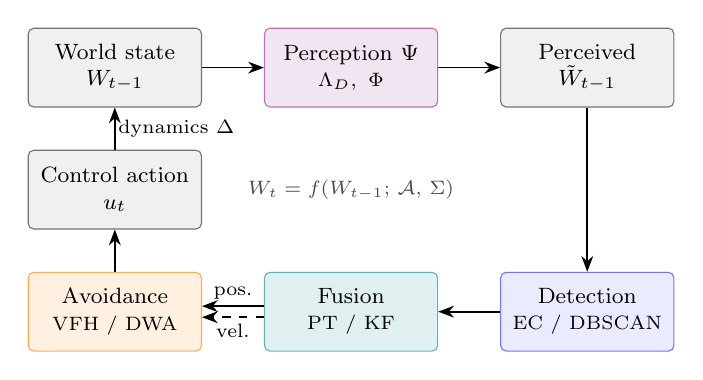
\begin{tikzpicture}[
  >={Stealth[length=2mm,width=1.5mm]},
  font=\footnotesize,
  box/.style={draw, rounded corners=2pt, align=center, inner sep=3pt,
              minimum width=22mm, minimum height=10mm, line width=0.4pt},
  world/.style={box, fill=black!6,     draw=black!55},
  perc/.style ={box, fill=violet!10,   draw=violet!55},
  det/.style  ={box, fill=blue!8,      draw=blue!55},
  fus/.style  ={box, fill=teal!12,     draw=teal!60},
  avo/.style  ={box, fill=orange!12,   draw=orange!65},
  ctrl/.style ={box, fill=black!6,     draw=black!55},
  arr/.style  ={->, semithick},
  arrd/.style ={->, semithick, dashed},
  sig/.style  ={font=\scriptsize, inner sep=1pt, align=center}
]
    % Top row: W_{t-1} -> Psi -> perceived world
    \node[world] (wt)     at (0, 3.1)  {World state\\$W_{t-1}$};
    \node[perc]  (psi)    at (3, 3.1)  {Perception $\Psi$\\{\scriptsize $\Lambda_D,\ \Phi$}};
    \node[world] (wtilde) at (6, 3.1)  {Perceived\\$\tilde{W}_{t-1}$};
    
    % Left column middle: control action
    \node[ctrl]  (c)      at (0, 1.55) {Control action\\$u_t$};
    
    % Bottom row (reversed order left-to-right to avoid crossings)
    \node[avo]   (a)      at (0, 0)    {Avoidance\\{\scriptsize VFH / DWA}};
    \node[fus]   (f)      at (3, 0)    {Fusion\\{\scriptsize PT / KF}};
    \node[det]   (d)      at (6, 0)    {Detection\\{\scriptsize EC / DBSCAN}};
    
    % Top-row arrows
    \draw[arr] (wt)  -- (psi);
    \draw[arr] (psi) -- (wtilde);
    
    % Right column: straight vertical down
    \draw[arr] (wtilde) -- (d);
    
    % Bottom row: right-to-left (Detection -> Fusion -> Avoidance)
    \draw[arr] (d) -- (f);
    
    % Fusion -> Avoidance: split into pos (solid, both) and vel (dashed, DWA-only)
    \draw[arr]  ([yshift=2pt]f.west) --
      node[above=-1pt, font=\scriptsize]{pos.} ([yshift=2pt]a.east);
    \draw[arrd] ([yshift=-2pt]f.west) --
      node[below=-1pt, font=\scriptsize]{vel.} ([yshift=-2pt]a.east);
    
    % Left column: straight vertical up (Avoidance -> Control -> World state)
    \draw[arr] (a) -- (c);
    \draw[arr] (c) -- node[right, sig]{dynamics $\Delta$} (wt);
    
    % One-step equation label inside the loop
    \node[sig, text=black!70] at (3, 1.55) {$W_t = f(W_{t-1};\,\mathcal{A},\,\Sigma)$};
\end{tikzpicture}
\caption{Simulation engine: one step of the core simulation loop~\eqref{eq:sim-function}.}
\label{fig:se-loop}
\vspace{-10px}
\end{figure}
 
The \texttt{SE} is governed by a parameter set $\Sigma$:
\begin{equation}
\label{eq:sigma}
    \Sigma = \langle \Lambda,\; \Phi,\; \Delta \rangle.
\end{equation}

\subsubsection{LiDAR sensor parameters $\Lambda$}
\label{sec:lidar-params}
The LiDAR parameters are partitioned into two subsets $\Lambda = \langle \Lambda_{\mathcal{S}},\; \Lambda_{\mathcal{D}} \rangle$:
 
The \emph{geometric parameters} $\Lambda_{\mathcal{S}}$:
\begin{itemize}
    \item $r_{\min}, r_{\max} \in \mathbb{R}^+$ --- minimum and maximum detection ranges.
    \item $\theta_{\text{fov}} \in (0, 2\pi]$ --- angular FOV.
    \item $\delta_\theta \in \mathbb{R}^+$ --- angular resolution.
    \item $f_{\text{scan}} \in \mathbb{R}^+$ --- scan frequency (Hz).
\end{itemize}
 
The \emph{distortion parameters} $\Lambda_{\mathcal{D}}$:
\begin{itemize}
    \item $\sigma_r \geq 0$ --- additive Gaussian range noise: $\hat{r}_j = r_j + \epsilon_j$, with $\epsilon_j \sim \mathcal{N}(0, \sigma_r^2)$.
    \item $p_{\text{miss}} \in [0, 1)$ --- probability that a ray returns no reading despite a surface being in range.
    \item $p_{\text{ghost}} \in [0, 1)$ --- probability of a spurious reading with no real surface.
\end{itemize}
 
\subsubsection{Perception and fusion parameters $\Phi$}
\begin{itemize}
    \item $\eta_{\text{cpl}} \in [0, 1]$ --- map completeness. The fraction of boundary elements in $E$ that are represented in the AGV's prior map. A value of $\eta_{\text{cpl}} = 1$ yields a perfect map; lower values simulate stale or incomplete maps.
    \item $\sigma_{\text{map}} \geq 0$ --- map noise. The positional perturbation applied to boundary elements in the prior map, modeling mapping inaccuracies.
\end{itemize}
 
The prior map $M_0$ is derived from $E$ as part of the perception function using the degradation parameters $\eta_{\text{cpl}}$ and $\sigma_{\text{map}}$ above. During simulation, the \texttt{SE} additionally maintains a runtime map $M_t$ that evolves as the fusion stage integrates new sensor observations with $M_0$. The runtime map is engine-internal state: it is not part of either $W_t$ or $\tilde{W}_t$, but is available to the fusion stage at each step.
 
\subsubsection{Simulation dynamics parameters $\Delta$} include $v_{\text{agv}}^{\max} \in \mathbb{R}^+$ --- maximum AGV velocity; $a_{\text{agv}}^{\max} \in \mathbb{R}^+$ --- maximum AGV acceleration; $\omega_{\text{agv}}^{\max} \in \mathbb{R}^+$ --- maximum AGV angular velocity; and $T_{\text{horizon}} \in \mathbb{R}^+$ --- maximum simulation duration.
 
% ============================================================
 
\section{Experimental Design}
\label{sec:experimental-design}
 
For every combination of initial world $W_0^{(i)} \in \mathcal{C}$, pipeline $\mathcal{A}^{(j)} \in \mathbb{A}$, and simulation configuration $\Sigma^{(k)} \in \mathbb{S}$, a simulation run $\texttt{SE}(W_0^{(i)}, \mathcal{A}^{(j)}, \Sigma^{(k)}, s_{\text{se}}^{(i,j,k)}) \to \mathcal{M}^{(i,j,k)}$ is executed and metrics are recorded. The protocol proceeds as: (1)~generate the world corpus $\mathcal{C}$; (2)~run all $(W_0, \mathcal{A}, \Sigma)$ triples; (3)~aggregate metrics; (4)~perform the validation analyses.

\begin{table}[t]
    \caption{World generation parameters}
    \label{tab:gen-params}
    \begin{center}
        \centering
        \begin{tabular}{|l|l|}
            \hline
            \textbf{Parameter} & \textbf{Values} \\
            \hline
            \multicolumn{2}{|l|}{\emph{Environment ($\Omega_{\text{env}}$)}} \\
            \hline
            Dimensions $X \times Y$ & $30 \times 30$\,m \\
            BSP depth $d_{\text{bsp}}$ & 1,\; 2,\; 3 \\
            Min partition $s_{\min}^{w} \times s_{\min}^{h}$ & $6 \times 6$\,m \\
            Split ratio $\rho_{\text{split}}$ & $[0.3, 0.7]$ \\
            Room padding $p_{\text{room}}$ & $[0.15, 0.35]$ \\
            Min corridor $c_{\min}$ & 2.0\,m \\
            Passage width $w_{\text{pass}}$ & 4.0\,m \\
            Wall thickness $t_{\text{wall}}$ & 0.3\,m \\
            \hline
            \multicolumn{2}{|l|}{\emph{AGV ($\Omega_{\text{agv}}$)}} \\
            \hline
            Body $L_{\text{agv}} \times W_{\text{agv}}$ & $0.6 \times 0.4$\,m \\
            \hline
            \multicolumn{2}{|l|}{\emph{Path ($\Omega_{\text{path}}$)}} \\
            \hline
            PRM samples $n_{\text{samples}}$ & 500 \\
            Neighbors $k_{\text{nn}}$ & 10 \\
            Max edge $l_{\max}$ & 5.0\,m \\
            Wall clearance $d_{\text{clear}}$ & 0.5\,m \\
            Min path length $l_{\pi}^{\min}$ & 15.0\,m \\
            Target speed $v^{\star}$ & 1.0\,m/s (const.) \\
            \hline
            \multicolumn{2}{|l|}{\emph{Obstacles ($\Omega_{\text{obs}}$)}} \\
            \hline
            Static count $n_{\text{static}}$ & 0,\; 4,\; 8,\; 16 \\
            Dynamic count $n_{\text{dynamic}}$ & 0,\; 2,\; 4,\; 8 \\
            Inscribed radius $\mathcal{D}_r$ & $\mathrm{Uniform}(0.1, 0.4)$\,m \\
            Min clearance $d_{\min}$ & 0.3\,m \\
            Obs.\ PRM samples & 300 \\
            Obs.\ speed $\mathcal{D}_v^{\text{obs}}$ & $\mathrm{Uniform}(0.2, 0.8)$\,m/s \\
            \hline
        \end{tabular}
    \end{center}
    \vspace{-7px}
\end{table}

\subsection{Pipeline Configurations}
\label{sec:pipeline-configs}
To validate the decomposition, we instantiate the three-stage pipeline $\mathcal{A} = \langle A_{\text{det}}, A_{\text{fus}}, A_{\text{avoid}} \rangle$ with two algorithms per stage, yielding $2 \times 2 \times 2 = 8$ configurations. All algorithms below are provided as built-in plugins in the released framework. Users may register additional algorithms via an abstract stage interface.
 
\subsubsection{Detection ($A_{\text{det}}$)}
The detection stage receives the distorted scan $\hat{L}_t$ and the prior map $M_0$, filters out points matching known boundary geometry, and groups remaining points into obstacle candidates:
\begin{itemize}
    \item \textbf{Euclidean Clustering (EC)}: groups points using a fixed distance threshold $d_{\text{ec}}$~\cite{rusu2011pcl}. Lightweight and widely used in AGV obstacle detection.
    \item \textbf{DBSCAN}: density-based clustering with neighborhood radius $\varepsilon$ and minimum cluster size. More robust to noise and varying obstacle densities~\cite{ester1996dbscan}.
\end{itemize}
 
\subsubsection{Fusion ($A_{\text{fus}}$)}
The fusion stage integrates current detections with historical observations:
\begin{itemize}
    \item \textbf{Pass-through (PT)}: no temporal fusion; $\bar{O}_t = \hat{O}_t$ directly. Minimal computation baseline. Because it does not estimate velocity, its output's velocity field is set to zero; downstream stages that consume this field hence operate under a stationary-obstacle assumption. 
    \item \textbf{Kalman Filter (KF)}: maintains position and velocity estimates per tracked obstacle using a constant-velocity model and nearest-neighbor association~\cite{welch1995kalman}.
\end{itemize}
 
\subsubsection{Avoidance ($A_{\text{avoid}}$)}
The avoidance stage computes a control action given the fused obstacle state and reference path:
\begin{itemize}
    \item \textbf{Vector Field Histogram (VFH)}: constructs a polar histogram of obstacle density and selects the best traversable direction~\cite{borenstein1991vfh}. It is worth noting that VFH is insensitive to velocity estimates from the fusion stage, as it considers only the obstacle's estimated position and radius.
    \item \textbf{Dynamic Window Approach (DWA)}: samples velocity pairs within kinematic constraints and selects the trajectory maximizing a weighted objective of heading, clearance, and speed~\cite{fox1997dwa}.
\end{itemize}
 
These configurations directly target RQ2: the permutation analysis (Section~\ref{sec:analyses}) holds two stages fixed and varies the algorithm at the target stage, isolating each stage's contribution to end-to-end performance.

\subsection{World Corpus}
\label{sec:corpus}
The world corpus $\mathcal{C}$ is generated by stratifying $\Omega$ across the values in Table~\ref{tab:gen-params}. The full factorial over BSP depth (3), static obstacle count (4), and dynamic obstacle count (4) yields $3 \times 4 \times 4 = 48$ strata. For each stratum, multiple worlds are generated with independent random seeds.

\subsection{Simulation Parameter Configurations}
\label{sec:sim-configs}
To assess result stability, we define a nominal simulation configuration and two degraded variants (Table~\ref{tab:sim-params}).
The \texttt{Nominal} configuration represents a well-calibrated LiDAR with a perfect prior map: the ``ideal'' operating condition. \texttt{Degraded-1} introduces moderate sensor noise, reduced range, and minor map incompleteness. \texttt{Degraded-2} represents a challenging scenario with significant noise, narrow FOV, coarse resolution, and a substantially incomplete map. The full $\Omega$ and $\Sigma$ parameter sets are exposed through YAML configuration files with documented defaults.

\begin{table}[htbp]
    \caption{Simulation parameter configurations}
    \label{tab:sim-params}
    \begin{center}
        \begin{tabular}{|l|c|c|c|}
            \hline
            \textbf{Parameter} & \textbf{\texttt{Nominal}} & \textbf{\texttt{Degraded-1}} & \textbf{\texttt{Degraded-2}} \\
            \hline
            \multicolumn{4}{|l|}{\emph{LiDAR geometric ($\Lambda_{\mathcal{S}}$)}} \\
            \hline
            $r_{\max}$ & 10\,m & 5\,m & 5\,m \\
            $r_{\min}$ & 0.05\,m & 0.05\,m & 0.05\,m \\
            $\theta_{\text{fov}}$ & $270^{\circ}$ & $270^{\circ}$ & $180^{\circ}$ \\
            $\delta_\theta$ & $0.5^{\circ}$ & $1^{\circ}$ & $2^{\circ}$ \\
            $f_{\text{scan}}$ & 15\,Hz & 15\,Hz & 10\,Hz \\
            \hline
            \multicolumn{4}{|l|}{\emph{LiDAR distortion ($\Lambda_{\mathcal{D}}$)}} \\
            \hline
            $\sigma_r$ & 0 & 0.02\,m & 0.05\,m \\
            $p_{\text{miss}}$ & 0 & 0.02 & 0.05 \\
            $p_{\text{ghost}}$ & 0 & 0.01 & 0.02 \\
            \hline
            \multicolumn{4}{|l|}{\emph{Perception ($\Phi$)}} \\
            \hline
            $\eta_{\text{cpl}}$ & 1.0 & 0.9 & 0.7 \\
            $\sigma_{\text{map}}$ & 0 & 0.05\,m & 0.1\,m \\
            \hline
            \multicolumn{4}{|l|}{\emph{Dynamics ($\Delta$)}} \\
            \hline
            $v_{\text{agv}}^{\max}$ & 1.5\,m/s & 1.5\,m/s & 1.5\,m/s \\
            $a_{\text{agv}}^{\max}$ & 1.0\,m/s$^2$ & 1.0\,m/s$^2$ & 1.0\,m/s$^2$ \\
            $\omega_{\text{agv}}^{\max}$ & 1.0\,rad/s & 1.0\,rad/s & 1.0\,rad/s \\
            $T_{\text{horizon}}$ & 120\,s & 120\,s & 120\,s \\
            \hline
        \end{tabular}
    \end{center}
    \vspace{-7px}
\end{table}

\subsection{Evaluation Metrics}
\label{sec:metrics}
For each simulation run, the following metrics are collected:
\begin{itemize}
    \item $\mu_{\text{col}}$ --- collision rate: fraction of runs in which the AGV collides with an obstacle or boundary.
    \item $\mu_{\text{dev}}$ --- path deviation: mean distance from the AGV's trajectory to the nearest segment of $\pi$.
    \item $\mu_{\text{goal}}$ --- goal reach rate: fraction of runs in which the AGV reaches $\mathbf{w}_n$ within $T_{\text{horizon}}$.
    \item $\mu_{\text{vel}}$ --- dynamic-obstacle velocity RMSE: root-mean-square error, averaged over dynamic obstacles and simulation steps, between the fusion-stage velocity estimate and the ground-truth velocity obtained from the obstacle's trajectory $\xi_i$.
    \item $\mu_{\text{comp}}$ --- computational cost: mean CPU time per simulation step.
    \item $\mu_{\text{lat}}$ --- latency: 95th-percentile per-step decision time.
\end{itemize}

\subsection{Validation Analyses}
\label{sec:analyses}
To address the outlined RQs, we perform the following analyses on the collected metrics:

\subsubsection{RQ1 --- Environment Realism}
For each generated world we compute the free-space ratio (fraction of $X\times Y$ not occupied by boundary geometry) and the minimum passage width (the narrowest gap between any two boundary segments on the AGV's reference path~$\pi$), and perform:
\begin{itemize}
    \item \textit{Parameter-consistency check:} free-space ratio should decrease monotonically with $d_{\text{bsp}}$, and the minimum passage width should cluster near $w_{\text{pass}}-t_{\text{wall}}$ by construction.
    \item \textit{Navigability-safety check:} the minimum passage width should exceed the AGV footprint plus clearance, $W_{\text{agv}}+2\,d_{\text{clear}}$, in every retained world.
    \item \textit{Difficulty-spread:} during the runs the $\mu_{\text{col}}$ and $\mu_{\text{dev}}$ should rise and $\mu_{\text{goal}}$ should fall with increasing obstacle count.
\end{itemize}

\subsubsection{RQ2 --- Decomposition Validity}
We run algorithm permutations over the three stages. A valid decomposition requires two properties: (i) \textit{direct stage sensitivity}, i.e., varying each algorithm primarily shifts its sensitivity-matched metric (detection $\to\mu_{\text{col}}$, fusion $\to\mu_{\text{vel}}$, avoidance $\to\mu_{\text{dev}},\mu_{\text{goal}}$); (ii) \textit{predictable stage interactions}, i.e., where an avoidance algorithm consumes a field produced by fusion (DWA's forward-prediction consumes the velocity field; VFH does not), the fusion-switch effect on avoidance-sensitive metrics should concentrate in the DWA-based pipelines. 

\begin{figure}[t]
    \centerline{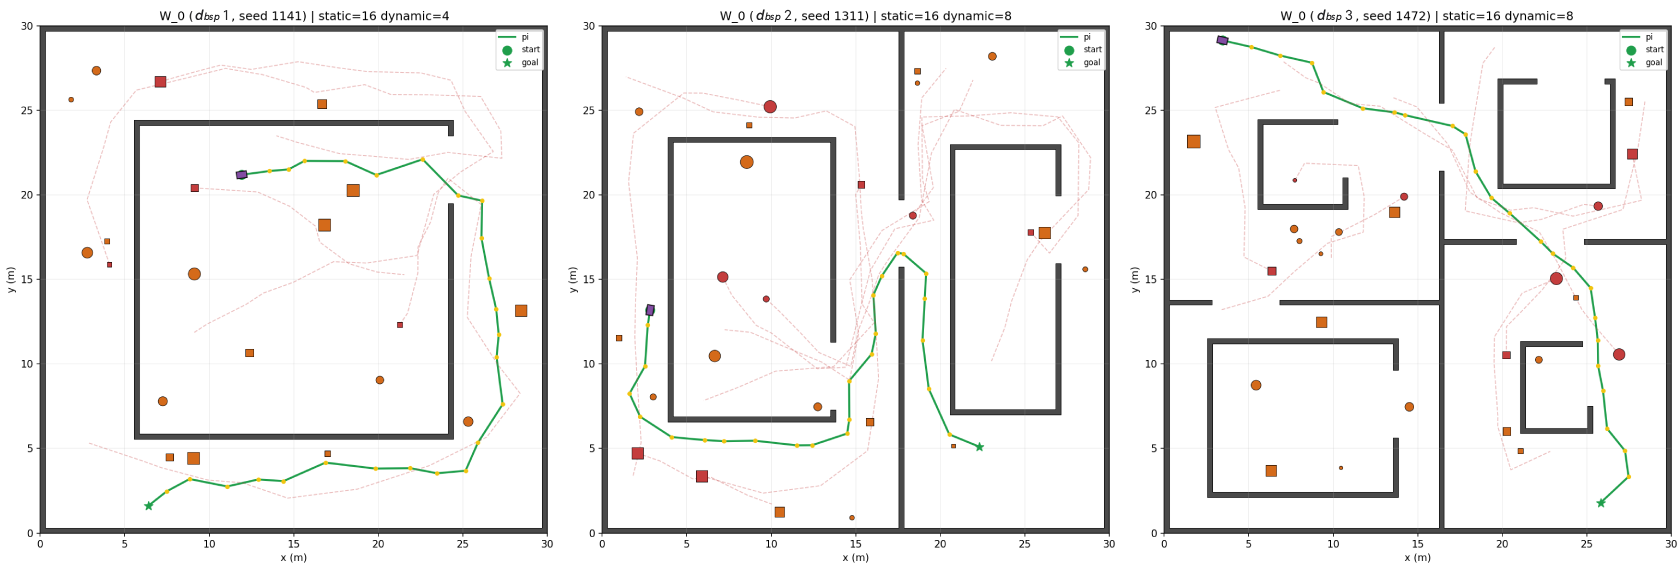
\includegraphics[width=\columnwidth]{img/example_worlds.png}}
    \caption{Example worlds generated at $d_{\text{bsp}} \in \{1, 2, 3\}$
    (left to right): environment boundaries $E$ (black), AGV reference path
    $\pi$ (green) with start (\textbullet) and goal ($\star$), static obstacles
    (orange), dynamic obstacles
    (red) and dynamic-obstacle trajectories (red, dashed).}
    \label{fig:example-worlds}
\end{figure}

\subsubsection{RQ3 --- Result Stability}
We compute the ranking of the 8 pipeline configurations under varying conditions, and perform:
\begin{itemize}
    \item \textit{Seed-stability check:} under the \texttt{Nominal} configuration, rankings should agree across disjoint subsets of $\mathcal{C}$, confirming that the benchmark's verdict does not depend on the particular draw of world seeds.
    \item \textit{Sensor-and-map-axis stability check:} per-metric rankings should persist across $\Sigma^{(k)}$; breakdowns on a particular metric localize the regime in which that metric's ranking is fragile.
\end{itemize}


 
\section{Results and Discussion}
\label{sec:results}
 
We instantiate the corpus $\mathcal{C}$ with $N=480$ worlds (10 per stratum over the 48 strata of Table~\ref{tab:gen-params}) and execute every $(W_0, \mathcal{A}, \Sigma)$ triple, producing $480 \times 8 \times 3 = 11{,}520$ runs.
Figure~\ref{fig:example-worlds} shows three representative outputs of the \texttt{WG}.
As can be observed, the same generator produces layouts from open halls to room-based facilities.
Table~\ref{tab:aggregate} summarizes the aggregate metrics; subsequent subsections analyze them against each research question.
 
\begin{table*}[htbp]
    \caption{Aggregate metrics across the 8 pipelines, with each metric reported under the three simulation configurations (means over $\mathcal{C}$)}
    \label{tab:aggregate}
    \begin{center}
        \setlength{\tabcolsep}{3pt}
        \footnotesize
        \begin{tabular}{|l|ccc|ccc|ccc|ccc|ccc|ccc|}
            \hline
            & \multicolumn{3}{c|}{$\mu_{\text{col}}$}
            & \multicolumn{3}{c|}{$\mu_{\text{dev}}$}
            & \multicolumn{3}{c|}{$\mu_{\text{goal}}$}
            & \multicolumn{3}{c|}{$\mu_{\text{vel}}$}
            & \multicolumn{3}{c|}{$\mu_{\text{comp}}$}
            & \multicolumn{3}{c|}{$\mu_{\text{lat}}$} \\
            \textbf{Pipeline}
            & N & D1 & D2 & N & D1 & D2 & N & D1 & D2 & N & D1 & D2 & N & D1 & D2 & N & D1 & D2 \\
            \hline
 
            EC + PT + VFH & 0.144 & 0.204 & 0.200 & 0.090 & 0.200 & 0.144 & 0.858 & 0.696 & 0.721 & 0.463 & 0.451 & 0.451 & 0.051 & 0.026 & 0.011 & 0.011 & 0.005 & 0.003 \\
            EC + PT + DWA & 0.450 & 0.404 & 0.342 & 0.332 & 0.290 & 0.279 & 0.438 & 0.352 & 0.329 & 0.454 & 0.434 & 0.423 & 0.074 & 0.040 & 0.026 & 0.056 & 0.038 & 0.042 \\
            EC + KF + VFH & 0.146 & 0.208 & 0.190 & 0.090 & 0.173 & 0.149 & 0.856 & 0.717 & 0.723 & 0.437 & 0.456 & 0.527 & 0.049 & 0.024 & 0.010 & 0.010 & 0.004 & 0.003 \\
            EC + KF + DWA & 0.410 & 0.344 & 0.310 & 0.351 & 0.304 & 0.300 & 0.487 & 0.383 & 0.356 & 0.429 & 0.428 & 0.460 & 0.078 & 0.041 & 0.028 & 0.062 & 0.041 & 0.042 \\
            DB + PT + VFH & 0.146 & 0.198 & 0.217 & 0.091 & 0.200 & 0.153 & 0.856 & 0.700 & 0.698 & 0.463 & 0.452 & 0.448 & 0.061 & 0.053 & 0.033 & 0.049 & 0.059 & 0.049 \\
            DB + PT + DWA & 0.448 & 0.375 & 0.327 & 0.332 & 0.300 & 0.268 & 0.440 & 0.377 & 0.304 & 0.453 & 0.433 & 0.408 & 0.089 & 0.073 & 0.051 & 0.096 & 0.089 & 0.082 \\
            DB + KF + VFH & 0.140 & 0.200 & 0.219 & 0.091 & 0.203 & 0.158 & 0.863 & 0.702 & 0.696 & 0.436 & 0.451 & 0.554 & 0.062 & 0.054 & 0.036 & 0.051 & 0.061 & 0.054 \\
            DB + KF + DWA & 0.410 & 0.338 & 0.323 & 0.349 & 0.311 & 0.300 & 0.485 & 0.425 & 0.331 & 0.429 & 0.424 & 0.479 & 0.087 & 0.070 & 0.050 & 0.092 & 0.086 & 0.080 \\
            \hline
        \end{tabular}
        \\[3pt]
        \raggedright
        \footnotesize
        DB = DBSCAN, N = \texttt{Nominal}, D1 = \texttt{Degraded-1}, D2 = \texttt{Degraded-2}.
    \end{center}
    \vspace{-10px}
\end{table*}
 
\subsection{Environment Realism}
\label{sec:results-rq1}
 
Figure~\ref{fig:rq1-distributions} shows the distributions of free-space ratio and minimum passage width across $\mathcal{C}$, grouped by BSP depth.
\begin{figure}[htbp]
\centerline{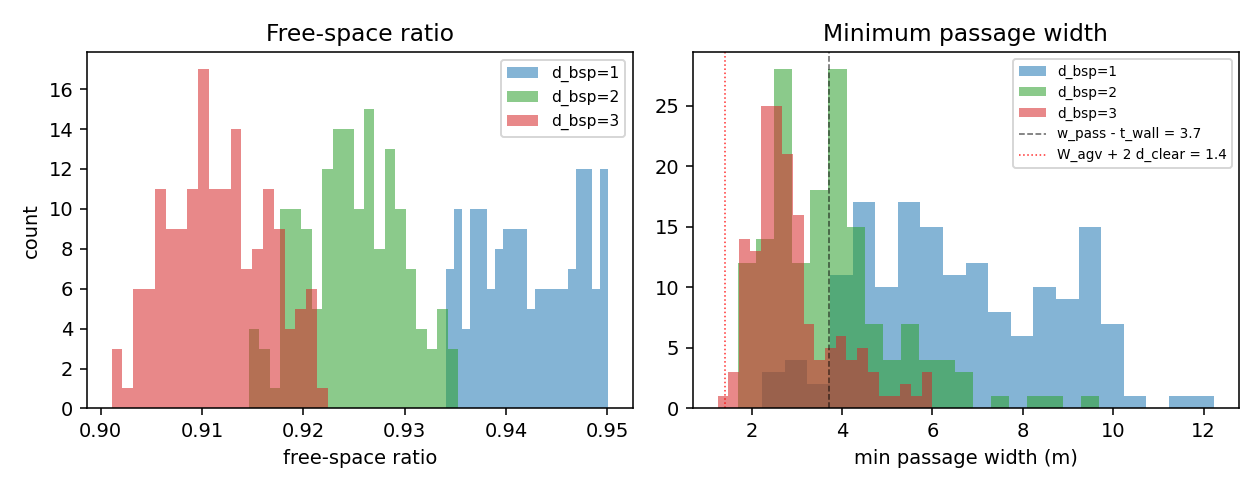
\includegraphics[width=\columnwidth]{img/rq1_distributions.png}}
\caption{Distributions of free-space ratio (left) and minimum passage width (right) across $\mathcal{C}$, stratified by $d_{\text{bsp}} \in \{1, 2, 3\}$.}
\label{fig:rq1-distributions}
\end{figure}
The mean free-space ratio is 0.942, 0.925, and 0.912 for $d_{\text{bsp}} = 1, 2, 3$ respectively, confirming the expected monotonic decrease. The minimum passage width concentrates at $\approx$\,4.41\,m, near the theoretical $w_{\text{pass}} - t_{\text{wall}} = 3.7$\,m.
With $W_{\text{agv}} + 2\,d_{\text{clear}} = 1.4$\,m, 99.8\,\% of generated worlds satisfy the clearance bound; worlds violating it are retained and inspected.
Figure~\ref{fig:rq1-difficulty} shows the travel metrics as functions of $n_{\text{static}}$ and $n_{\text{dynamic}}$, averaged over all \texttt{Nominal} runs. 

\begin{figure}[htbp]
    \centerline{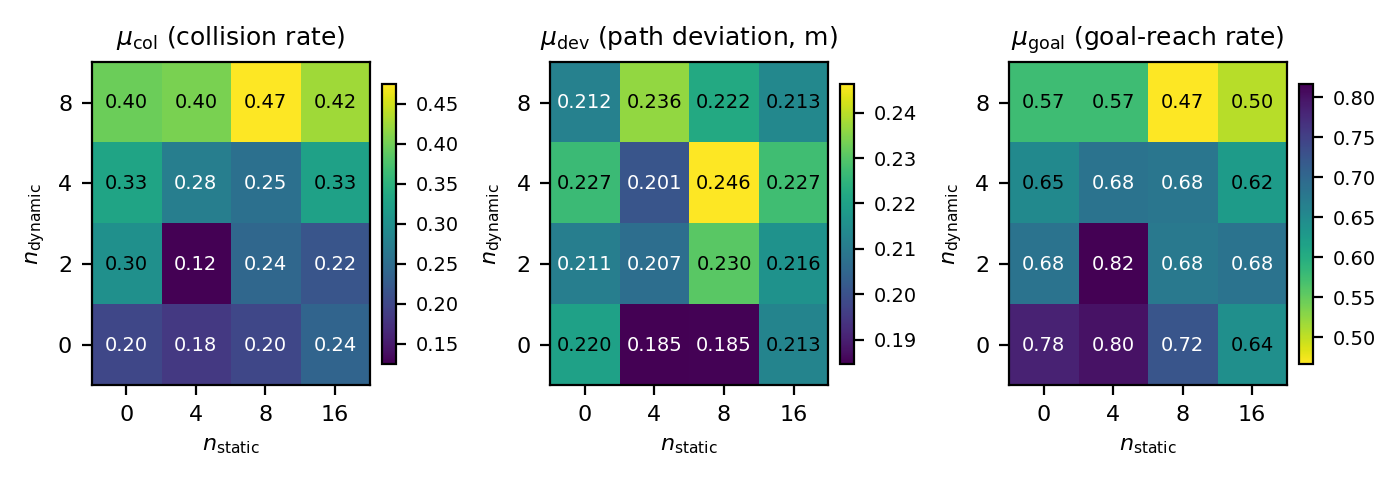
\includegraphics[width=\columnwidth]{img/rq1_difficulty.png}}
    \caption{Travel metrics as a function of obstacle counts under \texttt{Nominal}. Each cell aggregates the mean over all 8 pipelines and 10 world seeds in the $(n_{\text{static}}, n_{\text{dynamic}})$ stratum.}
    \label{fig:rq1-difficulty}
\end{figure}

Spearman correlations identify $n_{\text{dynamic}}$ as the dominant difficulty axis ($\rho=+0.182$ with $\mu_{\text{col}}$ and $\rho=-0.160$ with $\mu_{\text{goal}}$, both $p<10^{-3}$), while $n_{\text{static}}$ is comparatively flat at this scale with only $\mu_{\text{goal}}$ showing a small but significant $\rho=-0.061$ ($p<10^{-3}$); $\mu_{\text{col}}$ still spans 0.200--0.425 across the obstacle-count range.
Together, these checks support the interpretation that the corpus is well-formed, physically navigable, and spans a meaningful difficulty range.
 
\subsection{Decomposition Validity}
\label{sec:results-rq2}
 
Table~\ref{tab:rq2} reports the per-world median paired difference induced by switching each stage's algorithm, with the other two stages held fixed, under the \texttt{Nominal} configuration. Paired-difference significance is assessed with the two-sided Wilcoxon signed-rank test: for each table row the reported $p$ is the probability that a paired shift at least as large as the bolded $\Delta$ would arise under the null hypothesis that the algorithm switch has no effect on the bolded metric.
 
\begin{table}[htbp]
    \caption{Per-stage effects under algorithm permutation (\texttt{Nominal})}
    \label{tab:rq2}
    \begin{center}
        \begin{tabular}{|p{2.3cm}|p{0.727cm}|p{0.727cm}|p{0.727cm}|p{0.727cm}|p{0.947cm}|}
            \hline
            \textbf{Stage (switch)} & $\Delta\mu_{\text{col}}$ & $\Delta\mu_{\text{vel}}$ & $\Delta\mu_{\text{dev}}$ & $\Delta\mu_{\text{goal}}$ & $p$ \\
            \hline
 
            Detection (EC$\to$DB)       & \textbf{-0.002} & -0.000 & -0.000 & 0.001 & 0.439 \\
            Fusion (PT$\to$KF)          & -0.020 & \textbf{-0.026} & 0.009 & 0.025 & $<\!0.001$ \\
            $\mid$ Avoidance = VFH    & -0.002 & -0.027 & 0.000 & \textbf{0.002} & 0.715 \\
            $\mid$ Avoidance = DWA    & -0.039 & -0.025 & 0.018 & \textbf{0.048} & $<\!0.001$ \\
            Avoidance (VFH$\to$DWA)     & 0.286 & -0.009 & \textbf{0.251} & \textbf{-0.396} & $<\!0.001$ \\
            \hline
        \end{tabular}
        \\[3pt]
        \raggedright
        \footnotesize
        Median paired difference across $\mathcal{C}$. Bold entries denote the metric each row is expected to move: the stage's \emph{sensitivity-matched} metric for the three main rows, and the \emph{interaction-target} metric $\mu_{\text{goal}}$ for the two avoidance-sliced rows.
    \end{center}
\end{table}
 
Property~(i) partially holds: fusion and avoidance shift their sensitivity-matched metrics at $p<10^{-3}$, whereas detection's $\mu_{\text{col}}$ shift of $-0.002$ is below the statistical resolution of this corpus ($p=0.439$). Property~(ii) holds: the fusion-switch effect on $\mu_{\text{goal}}$ is $0.002$ ($p=0.715$) under VFH and $0.048$ ($p<10^{-3}$) under DWA, consistent with DWA's consumption of the velocity field and VFH's non-consumption. 
 
\subsection{Result Stability}
\label{sec:results-rq3}
 
Table~\ref{tab:rq3} reports Kendall's rank-correlation coefficient $\tau$ between pairs of per-metric pipeline rankings. The \emph{Seed (shards)} column is the mean pairwise $\tau$ over 3 disjoint \texttt{Nominal} seed shards (probing seed dependence); the remaining columns pairwise-compare rankings under \texttt{Nominal}, \texttt{Degraded-1}, and \texttt{Degraded-2} (probing sensor/map-degradation dependence).
 
Rankings are metric-dependent: the minimum pairwise $\tau = -0.286$ occurs for $\mu_{\text{vel}}$ on Nom--Deg2, while every other travel metric retains $\tau \geq 0.618$ on the same pair. A plausible mechanism is DWA's run-timeout rate, which rises from 10.8\% under \texttt{Nominal} to 34.4\% under \texttt{Degraded-2} (VFH stays below 10\%): DWA pipelines then accumulate fewer dynamic-obstacle tracking steps, re-weighting $\mu_{\text{vel}}$'s step-averaged RMSE in a way that does not track fusion quality. We interpret this as a regime-dependent sensitivity of $\mu_{\text{vel}}$, surfaced by the benchmark rather than a failure of it.

\begin{table}[htbp]
    \caption{Pairwise Kendall's $\tau$ between pipeline rankings per metric}
    \label{tab:rq3}
    \begin{center}
        \begin{tabular}{|l|c|c|c|c|}
            \hline
            \textbf{Metric} & \textbf{Seed (shards)} & \textbf{Nom–Deg1} & \textbf{Nom–Deg2} & \textbf{Deg1–Deg2} \\
            \hline
 
            $\mu_{\text{col}}$   & 0.715 & 0.815 & 0.667 & 0.571 \\
            $\mu_{\text{dev}}$   & 0.667 & 0.857 & 0.857 & 0.714 \\
            $\mu_{\text{goal}}$  & 0.707 & 0.691 & 0.618 & 0.643 \\
            $\mu_{\text{vel}}$   & 0.857 & 0.500 & -0.286 & 0.071 \\
            \hline
        \end{tabular}
        \\[3pt]
        \raggedright
        \footnotesize
        Values near $+1$ denote rank agreement; values near $-1$ denote reversal. The Seed (shards) column is the mean over the 3 disjoint \texttt{Nominal} shard pairings; the remaining columns compare rankings between \texttt{Nominal}, \texttt{Degraded-1}, and \texttt{Degraded-2}.
    \end{center}
\end{table}

Pooling the Seed (shards) column yields an overall mean $\tau = 0.737$, indicating that the ranking is robust to the particular draw of world seeds.
 
 
\subsection{Discussion}
\label{sec:discussion}
The three analyses jointly support the framework's use as a benchmarking instrument: the corpus is well-formed and difficulty-graded (RQ1), the pipeline stages exhibit the intended sensitivity pattern and surface predicted stage interactions (RQ2), and rankings are stable enough for the benchmark's verdict to be reproducible (RQ3). Under \texttt{Nominal}, Table~\ref{tab:aggregate} additionally orders pipelines by cost: VFH runs at $\mu_{\text{comp}}\!\approx\!0.049$--$0.062$\,s and $\mu_{\text{lat}}\!\approx\!0.010$--$0.051$\,s versus DWA's $0.074$--$0.089$\,s and $0.056$--$0.096$\,s, and EC detection is consistently cheaper than DBSCAN at fixed fusion and avoidance (e.g., $\mu_{\text{comp}}=0.049$ vs.\ $0.062$\,s for KF+VFH). DWA's higher collision and timeout rates in this corpus reflect the algorithm's known sensitivity to objective-weight tuning rather than a general capability gap; surfacing such tuning sensitivity per stage and per regime is itself one of the framework's intended outputs. The 11{,}520-run sweep ran in $\sim$8 wall-clock hours on a 16-core workstation, scaling linearly with available cores since runs are independent. Where checks are only partially met, the framework's parameter-controlled design localizes the cause to a specific stage, metric, or regime, rather than leaving it as an uncharacterized source of variance --- which is the property that distinguishes a benchmarking instrument from a single-scenario evaluation.
 
Several limitations shape the scope of these results. First, as noted in Section~\ref{sec:perception-model}, the AGV's self-pose is treated as oracle-known inside $\tilde{W}_t$; real localization uncertainty (odometry drift, SLAM error) is not modeled here. Second, the RQ1 checks establish internal consistency and navigability rather than statistical equivalence to a specific empirical warehouse population, which would require curated measurements from real facilities. Sim-to-real transfer on a physical AGV testbed thus remains the principal question of external validity. Third, the framework currently models a single AGV, with multi-AGV coordination being a natural extension.
A pose-noise model, processing-latency modeling, large-scale algorithm benchmarking, per-stratum conditional analysis, sim-to-real transfer, and comparison with external simulators are planned for the journal extension.
 
\section{Conclusion}
\label{sec:conclusion}
 

In this work, we present a simulation-driven benchmarking framework for LiDAR-based collision avoidance on AGVs, comprising a parameterized procedural world generator and a modular three-stage simulation engine with an explicit sensor- and map-degradation model. Validation on a stratified corpus showed that the generated environments are well-formed and cover a meaningful difficulty range; that each pipeline stage shifts its intended metric in isolation, with detection below the corpus's statistical resolution; and that pipeline rankings are robust to world-seed resampling and largely stable across sensor and map degradation. Unlike a fixed dataset, the framework is a formal specification: it supports on-demand corpus regeneration, controlled stage substitution, and clean separation of perception-side from algorithmic failures. Planned extensions include AGV self-pose uncertainty, processing-latency modeling, per-stratum conditional analysis, integration of learned stages, and cross-simulator validation against external physics backends.

\section*{Acknowledgment}
Co-funded by the European Union HORIZON TMA MSCA Doctoral Networks / HORIZON-MSCA-2023-DN-01 / project TUAI / grant agreement N° 101168344. Views and opinions expressed are, however, those of the author(s) only and do not necessarily reflect those of the European Union or European Research Executive Agency. Neither the European Union nor the granting authority can be held responsible for them.

During the preparation of this work, the authors used \textit{Anthropic Claude Opus 4.7} for proofreading, text readability improvement, and partial code generation. After using this tool, the authors reviewed and edited the content as needed and take full responsibility for the content of the publication.
 
\bibliographystyle{IEEEtran}
\bibliography{ref}
 
\end{document}